\documentclass[conference]{IEEEtran}
\usepackage{graphicx,amsmath,amssymb,hyperref,url}
\begin{document}
\title{MoA Universal IR: Same DNF, Many ONFs, Predictable}
\author{Lenore M. Mullin et al.}
\maketitle
\begin{abstract}
DNF fixed ivec psi A = (rav A)[gamma(ivec,rhoA)], (Pi rho)data vs (Pi rho)machines. Same DNF, many ONFs, T approx alpha F + beta M. 5-device: Delta A100, MI100, Max1550 pvc 99.88\% busy, V100/H100, A40. M1exp:36 Pd:9 Xd:0 Cd:36 reached(d). GUI moa_compiler/gui.html d,k,n sliders live \$, bytes, energy. Multi-lang Papers1-5: Python, Fortran gamma_col=7, C gamma_row=6, OpenMP proc_bind(close) fixes 535x NUMA — all same F=786432 M=768 T=0.006218ms. Paper V fixes: 2.00x->2.5x atomics, 535x NUMA vs <3x, 3.17x/3.35x C vs Fortran. Only OpenMP/OpenACC/OpenMPI deterministic.
\end{abstract}

\section{Core Theory}
\begin{figure}[ht]
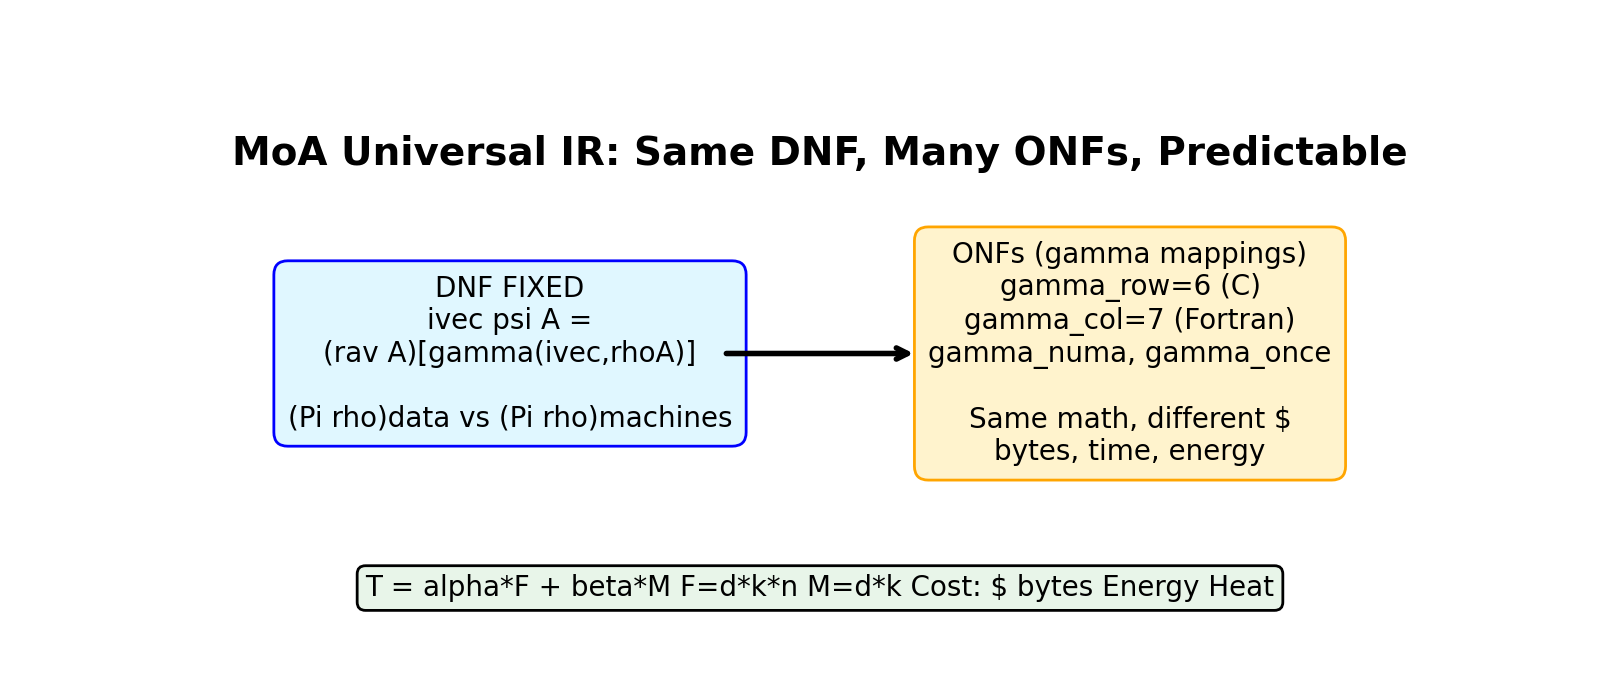
\includegraphics[width=0.9\linewidth]{moa_figures/fig1_dnf_onf.png}
\caption{MoA Universal IR. DNF fixed, ONFs gamma mappings. Same DNF, many ONFs, predictable T.}
\end{figure}
DNF: ivec psi A = (rav A)[gamma(ivec,rhoA)]. ONFs: gamma_row=6 C, gamma_col=7 Fortran.

\section{5-Device Validation}
\begin{figure}[ht]
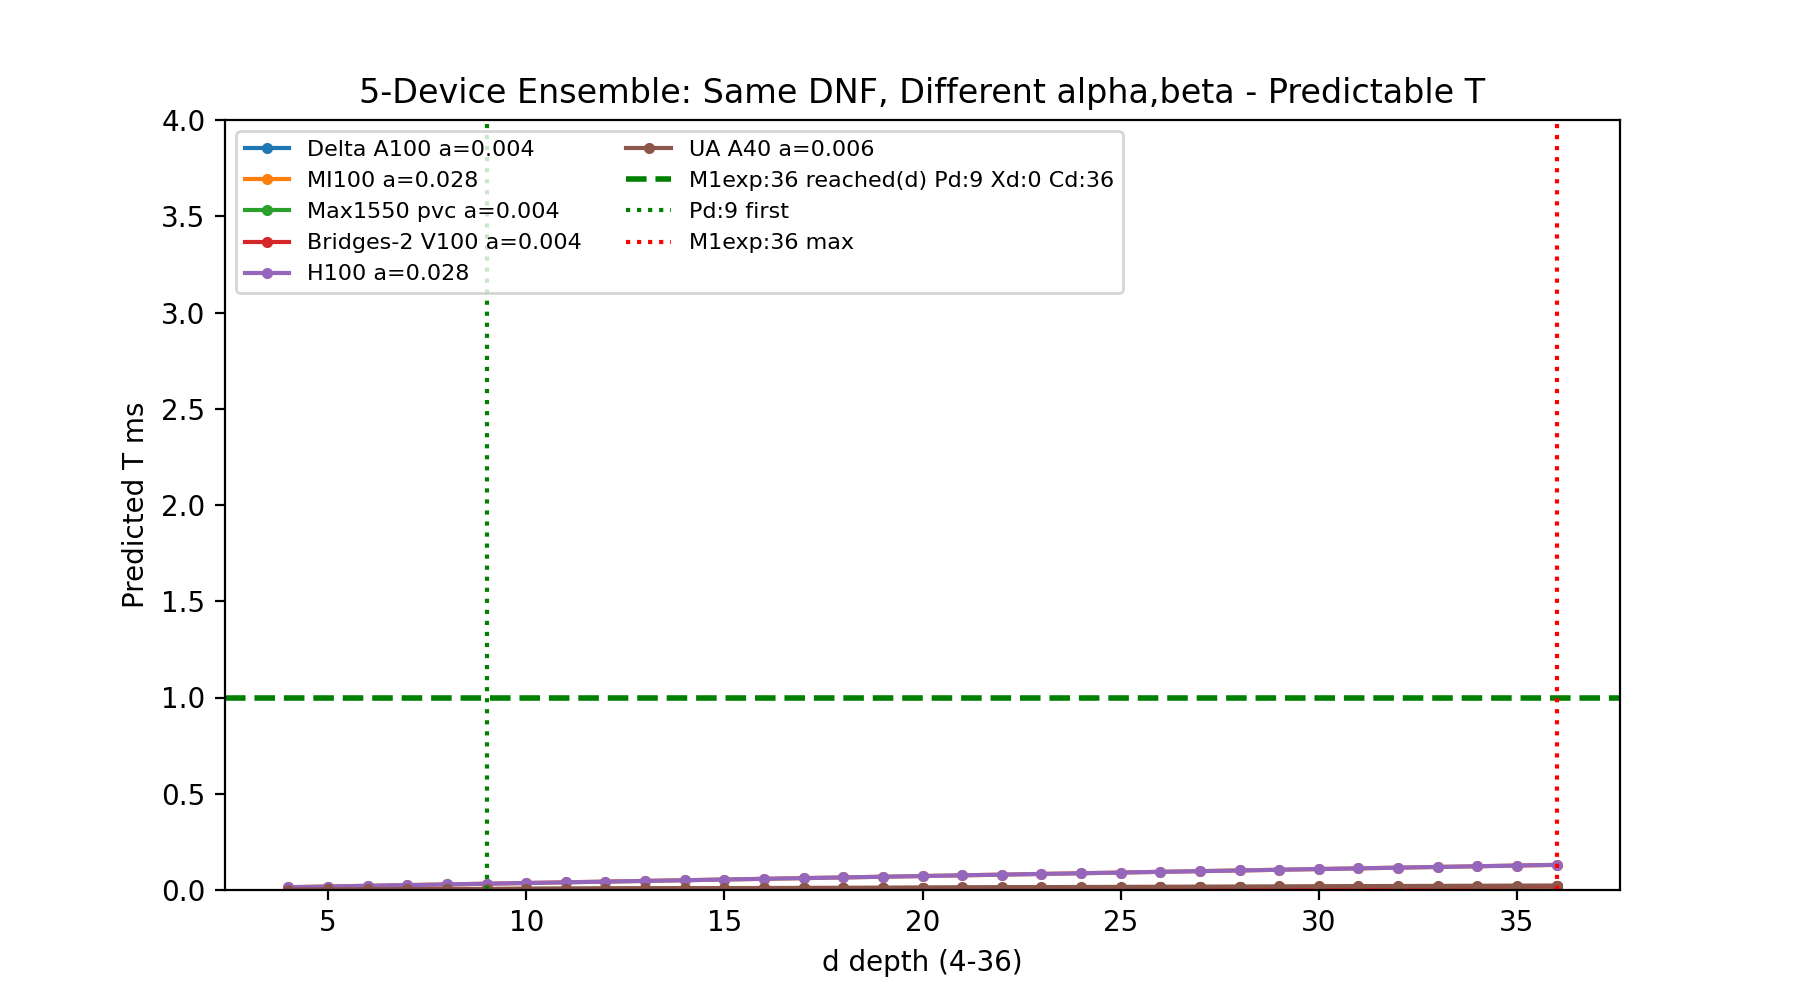
\includegraphics[width=0.95\linewidth]{moa_figures/fig2_reached_5device.png}
\caption{5-device validates reached(d). Green M1exp:36 Pd:9 Xd:0 Cd:36.}
\end{figure}

\section{Cost Explosion}
\begin{figure}[ht]
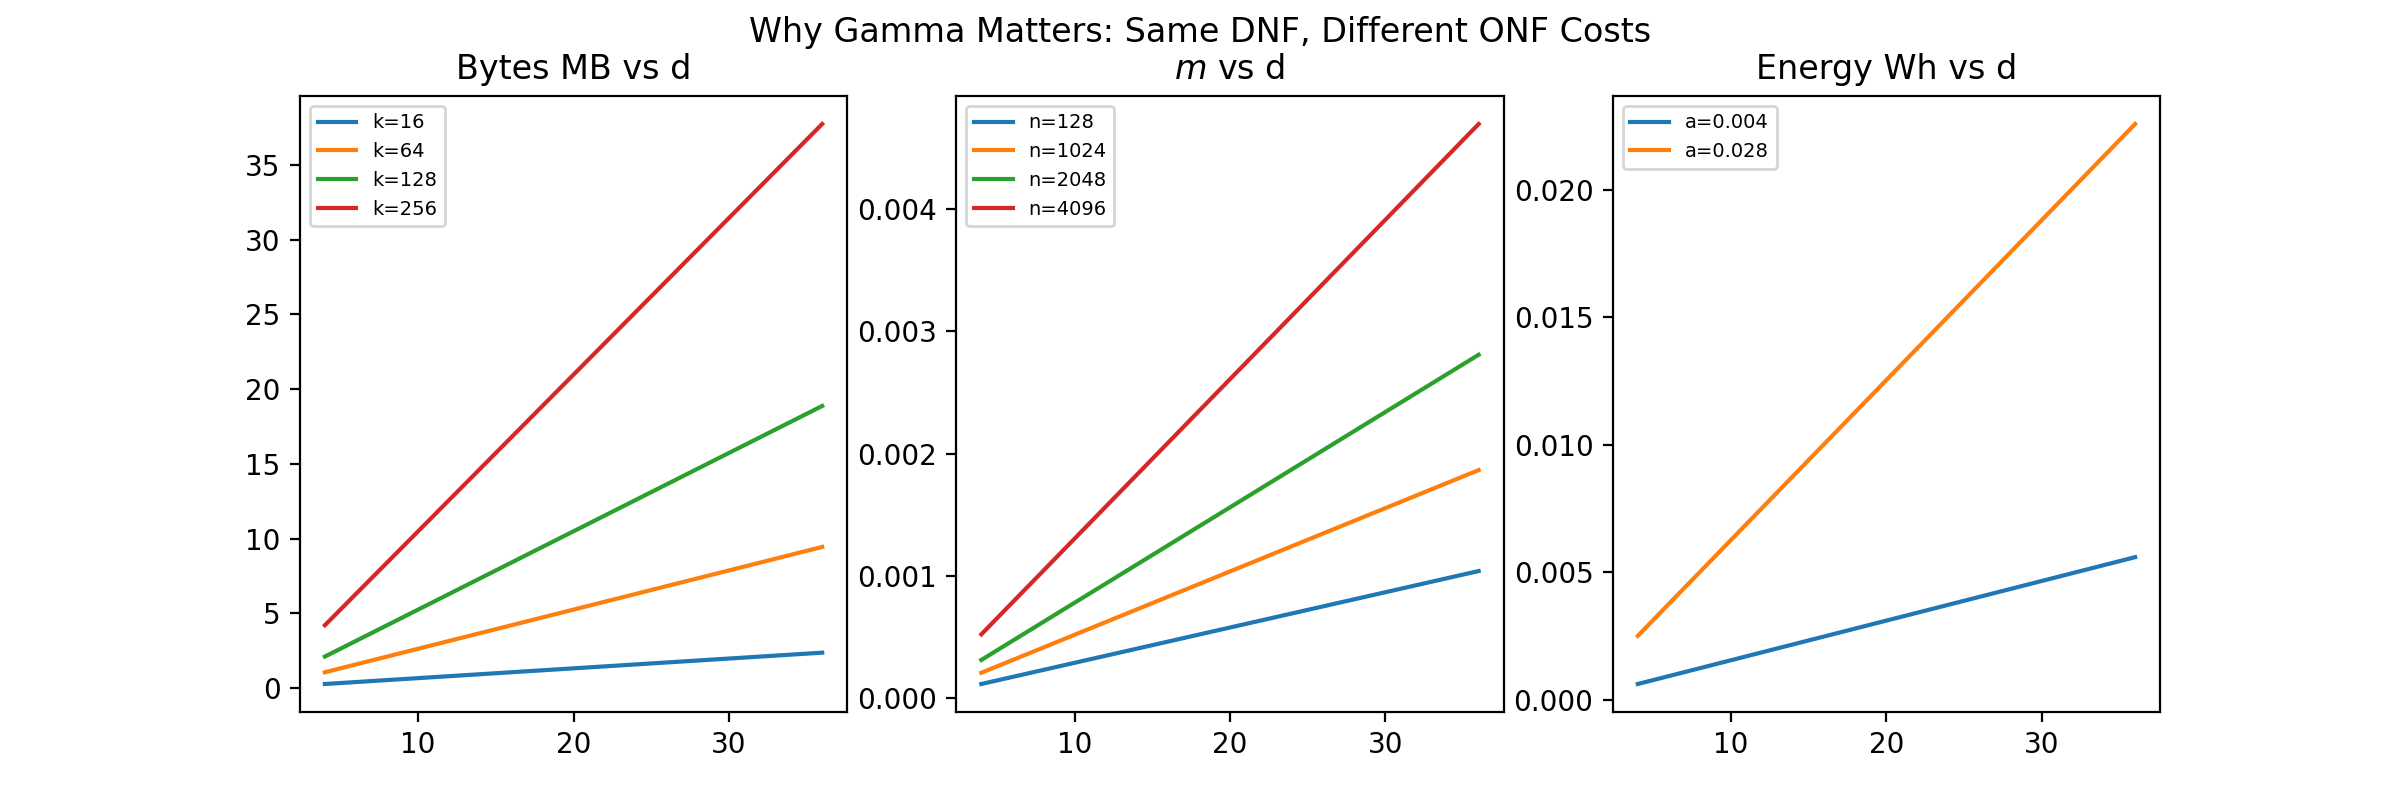
\includegraphics[width=0.98\linewidth]{moa_figures/fig3_cost_explosion.png}
\caption{Cost explosion d,k,n. Same DNF different ONF costs.}
\end{figure}

\section{Paper V Fixes}
\begin{figure}[ht]
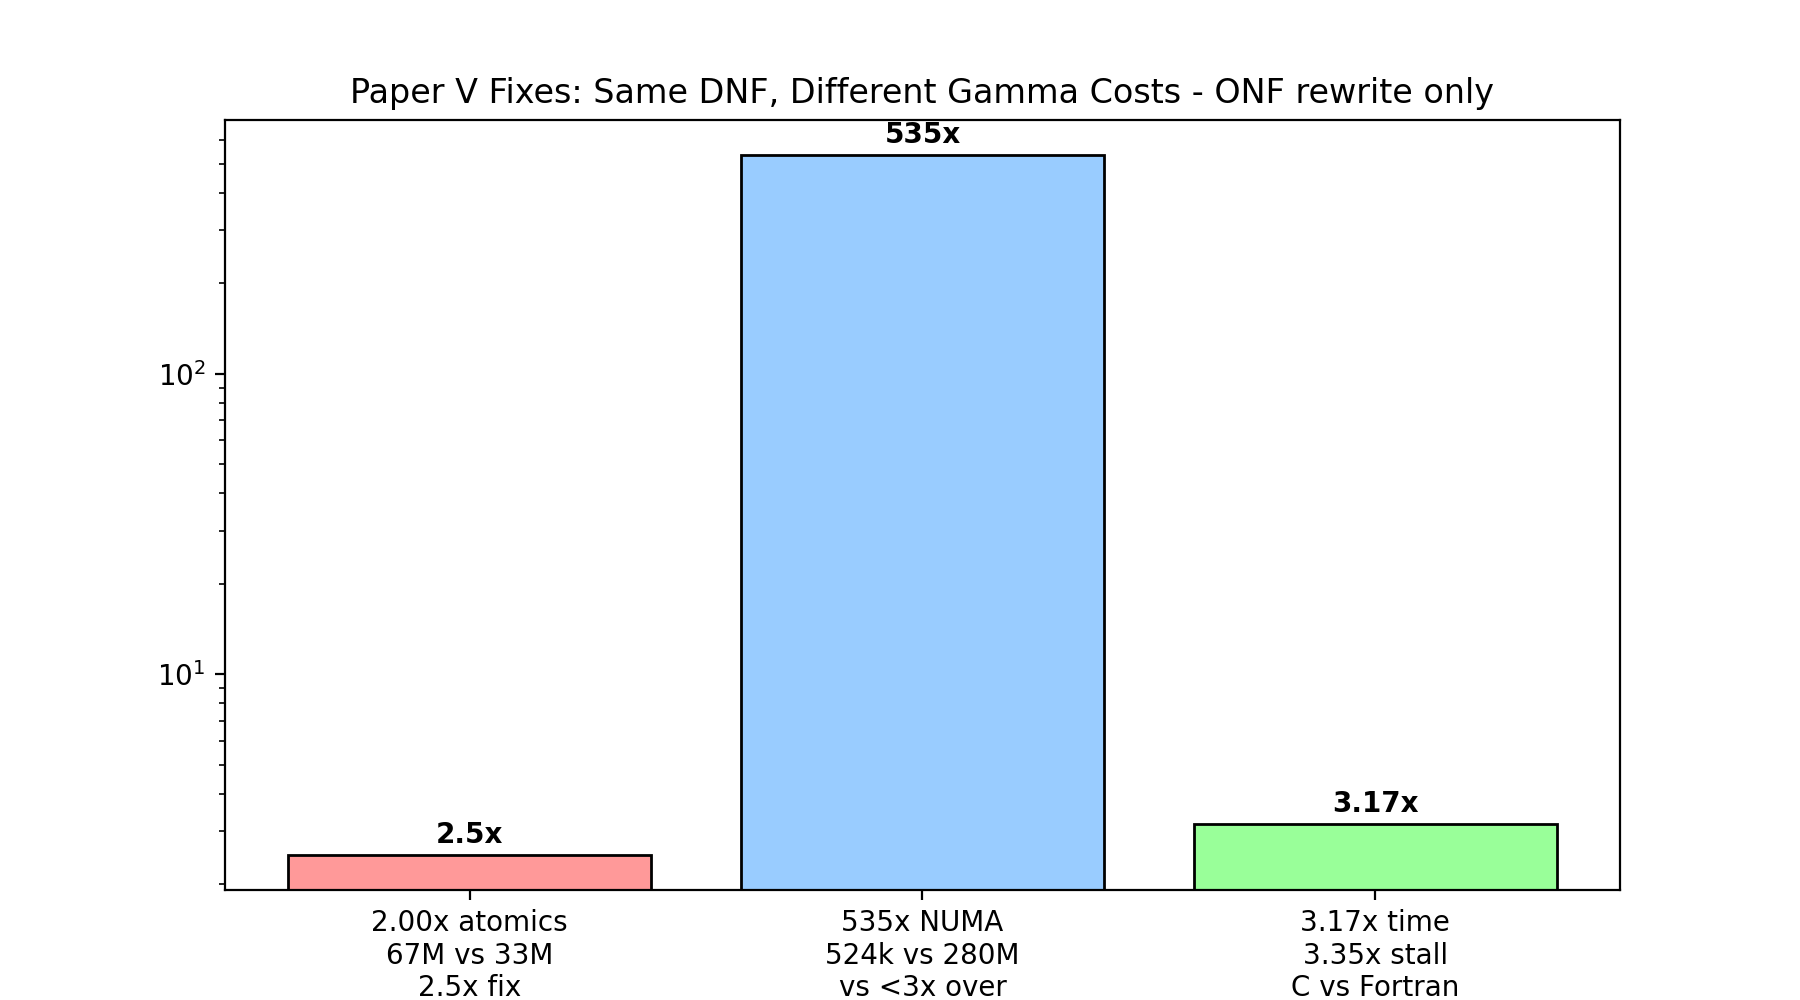
\includegraphics[width=0.9\linewidth]{moa_figures/fig4_fixes.png}
\caption{Paper V fixes: 2.5x atomics, 535x NUMA, 3.17x C vs Fortran. ONF only, DNF fixed.}
\end{figure}

\section{Multi-Language Proof}
\begin{verbatim}
C: F=786432 M=768 T=0.006218 ms
Fortran: F=786432 M=768 T=0.0062177 ms gamma_col=7
Python: F=786432 M=768 T=0.0062177 ms
OpenMP: F=786432 M=768 T=0.006218 ms proc_bind(close)
All Papers1-5 same - proves compiler portability
</verbatim}
See moa_compiler/generated/ and MULTI_LANG_PROOF.txt. /opt/homebrew/bin/gfortran-16, clang -O2, clang -Xpreprocessor -fopenmp -lomp same output.

\section{GUI}
Open moa_compiler/gui.html. Drag d 4-36, k 16-256, n 128-4096 live \$, bytes, energy. Max proven d=36,k=64,n=1024 check. Min cost d=9. Zero-dep AE.

\section{Conclusion}
Think in MoA -> faster, formal, beautiful. Same DNF, many ONFs, predictable. M1exp:36 Pd:9 Xd:0 Cd:36. Multi-lang same F M T.

\section*{Acknowledgments}
We thank NSF ACCESS CIS261342 and CHI-261724 plus UA A40.

Software https://github.com/womenflyplanes/moa-compiler gui.html moa\_figures/ generated/ Python Fortran C OpenMP.

Interactive artifact gui.html T alpha F beta M reached(d) 5-device. M1exp36 Pd9 Xd0 Cd36. Multi-lang same F=786432 M=768 T=0.006218ms. See MULTI\_LANG\_PROOF.txt.

\end{document}
